\documentclass[tikz]{standalone}

\usepackage{fontspec}

\usetikzlibrary{arrows}
\usetikzlibrary{calc}
\usetikzlibrary{decorations.pathreplacing}
\usetikzlibrary{positioning}
\usetikzlibrary{matrix}

\usepackage{fontspec}

\begin{document}

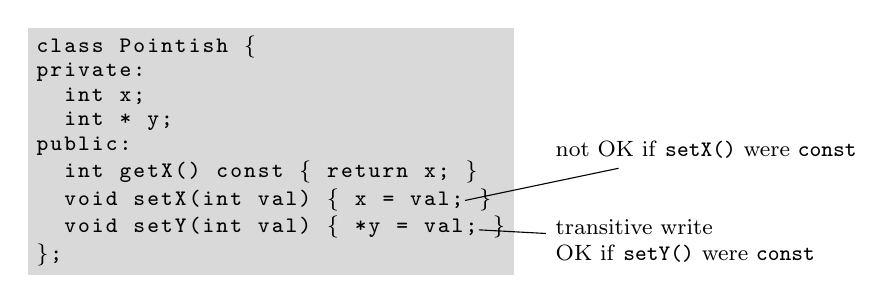
\begin{tikzpicture}
  [node distance=5mm, >=stealth',
  every node/.style={font=\footnotesize},
  every matrix/.style={fill=black!15, inner sep=1mm, row sep=0.5mm,
                        matrix of nodes, nodes in empty cells,
                        minimum height=0.5em, minimum width=.5em,
                        nodes={anchor=base, inner sep=0, font=\ttfamily\footnotesize}}]

  \matrix (Pointish) {
c & l & a & s & s &   & P & o & i & n & t & i & s & h &   & \{ &   &   &   &   &   &   &   &   &   &   &   &   &   &   &   &   &   &   \\
p & r & i & v & a & t & e & : &   &   &   &   &   &   &   &   &   &   &   &   &   &   &   &   &   &   &   &   &   &   &   &   &   &   \\
  &   & i & n & t &   & x & ; &   &   &   &   &   &   &   &   &   &   &   &   &   &   &   &   &   &   &   &   &   &   &   &   &   &   \\
  &   & i & n & t &   & * &   & y & ; &   &   &   &   &   &   &   &   &   &   &   &   &   &   &   &   &   &   &   &   &   &   &   &   \\
p & u & b & l & i & c & : &   &   &   &   &   &   &   &   &   &   &   &   &   &   &   &   &   &   &   &   &   &   &   &   &   &   &   \\
  &   & i & n & t &   & g & e & t & X & ( & ) &   & c & o & n & s & t &   & \{ &   & r & e & t & u & r & n &   & x & ; &   & \} &   &   \\
  &   & v & o & i & d &   & s & e & t & X & ( & i & n & t &   & v & a & l & ) &   & \{ &   & x &   & = &   & v & a & l & ; &   & \} &   \\
  &   & v & o & i & d &   & s & e & t & Y & ( & i & n & t &   & v & a & l & ) &   & \{ &   & * & y &   & = &   & v & a & l & ; &   & \} \\
\} & ; &   &   &   &   &   &   &   &   &   &   &   &   &   &   &   &   &   &   &   &   &   &   &   &   &   &   &   &   &   &   &   &   \\
  };

  \node (x)  [right=of Pointish-7-34, yshift=2em] {not OK if \texttt{setX()} were \texttt{\textbf{const}}};
  \node (y) [align=left, right=of Pointish-8-34,yshift=-.5em] {transitive write\\OK if \texttt{setY()} were \texttt{\textbf{const}}};

  \path (Pointish-7-31) edge (x)
        (Pointish-8-32) edge (y);
\end{tikzpicture}

\end{document}
